\documentclass[10pt, notes]{beamer}       % print frame + notes
% \documentclass[10pt, notes=only]{beamer}   % only notes
% \documentclass[12pt]{beamer}              % only frames

\usetheme[progressbar=frametitle]{metropolis}

\usepackage{booktabs}
\usepackage[scale=2]{ccicons}
\usepackage[export]{adjustbox}

\usepackage{pgfplots}
\usepgfplotslibrary{dateplot}

\usepackage{xspace}
\usepackage[backend=biber]{biblatex}
\addbibresource{bibliography.bib}
\usepackage{tikz}
\newcommand{\themename}{\textbf{\textsc{metropolis}}\xspace}

\newcommand{\redc}[2][red,fill=red]{\tikz[baseline=-0.5ex]\draw[#1,radius=#2] (0,0) circle ;}%
\newcommand{\bluec}[2][blue,fill=blue]{\tikz[baseline=-0.5ex]\draw[#1,radius=#2] (0,0) circle ;}%


% Set up table of contents
\AtBeginSection[]
{
\begin{frame}<beamer>
\frametitle{Outline}
\tableofcontents[
  currentsection,
  sectionstyle=show/shaded,
  subsectionstyle=show/show/hide
]
\end{frame}
}

% Make alert boxes have filled backgrounds
\metroset{block=fill}



\title{Simulation and Theory of Bacterial Transformation}
\date{August 5, 2016}
\author{JD Russo, JJ Dong}
\institute{Department of Physics and Astronomy\\Bucknell University}

\begin{document}

\maketitle

\section{Introduction}

\subsection{Motivation}
\begin{frame}{Motivation}
  \begin{itemize}
    \item Ubiquitous threat of antibiotic resistance
    \item Transmission of resistance via plasmids
    \item Identify what most significantly affects resistant cell dominance.
    %TODO: Something along the lines of "Investigating what gives rise to conditions
    % where antibiotic resistance dominates"
  \end{itemize}

  \vspace*{\fill}
    \begin{alertblock}{Question}
      What conditions lead to emergence of antibiotic resistance?
    \end{alertblock}
  \vspace*{\fill}

\end{frame}
\note[itemize]{
\item Threat of resistance even in well-controlled diseases (TB)
\item  Main mechanisms of transmission are conjugation and transformation
}



\subsection{Biological Background}
%TODO: Label this as Biological Background - Plasmids ?
\begin{frame}[fragile]{Plasmids}
  \begin{itemize}
    \item Small, independently replicating genetic material
    \item Often include DNA segments encoding antibiotic resistance
    \item Imposes a fitness cost on host cell
  \end{itemize}
\end{frame}

\begin{frame}{Transformation and Conjugation}

  \begin{itemize}
    \item \textbf{Transformation:} Cell incorporates plasmid from environment
    \item \textbf{Conjugation:} Plasmid transferred between cells
  \end{itemize}

  \vspace*{\fill}
  \centerline{\includegraphics[width=.5\paperwidth]{../../dev/graphics/poster/transformation.pdf}}
  % \vspace*{\fill}
\end{frame}
\note[itemize]{
\item Transformation is the process where a cell incorporates a plasmid from its
environment, translating any encoded genes
\item Conjugation is horizontal transfer of a plasmid between two cells
\item We assume transformation is the primary mechanism of plasmid transfer because
we also assume that when a cell acquires a plasmid, it keeps it.
}



\section{Simulation}
%TODO: Should this go here?
\begin{frame}{Simulation vs Modeling}
  \begin{itemize}
  \item Stochastic vs Deterministic
  \item Information about average behavior vs specific trajectories
  \item Individual realizations noisily follow model
  \end{itemize}
  \vfill
  %TODO: Anderson's figure is a lot better - shows cases where a pop completely
  % dies off, i.e. where a certain trajectory has vastly different behavior even
  % in the limit of long time
  \centerline{\includegraphics[width=.7\paperwidth]{../../dev/graphics/talk/trajectories.pdf}}
\end{frame}
\note[itemize]{
\item At a very general level... More general discussion of models vs simulations
\item Mathematical modeling of populations is deterministic - useful to capture info about average behavios
\item Simulations can incorporate stochastic reactions
\item If any of you remember, both Jonathan and Josh have mentioned generalizing from
discrete to continuum limits. In our case we can get more information about population growth
by doing the opposite, moving from a continuous model,
the differential equations that describe general behavior of populations, to
the discrete simulation, which model behavior of individual populations.
\item Individual experiments noisily follow model
}
%TODO: Is the flow from the introduction of simulation into the population equations into the KMC good? Should I do KMC then DE?
\begin{frame}{Simulation vs Modeling}

  \begin{align}
    \uncover<1->{&\text{Reaction} & \quad & R \stackrel{\delta}{\longrightarrow} \varnothing \\}
    \uncover<2->{
      &\text{Differential equation}&&\frac{dR}{dt} = - \delta R\\
      &&& R(t) = R_0  e^{- \delta t} \\
    }
    \notag
  \end{align}

  % \vspace*{\fill}
\end{frame}
\note[itemize]{ %TODO: Fact check this with JJ
%TODO: i'm repeating myself about the simulation vs model thing here \ No, I'm giving an example of what I mean
\item This reaction describes a basic situation where a resistant cell dies with
probability $\delta$.
\item You can phrase this mathematically by writing the differential equation
\item ... Which you can solve to find the exact solution for the population at any time
\item Plotting this equation describes an exponential function that symptotically
  approaches zero.
\item However, implementing this reaction in simulation, this is not a smooth curve. This is a step-like function,
  where for instance at some discrete time the population jumps from one to zero and goes extinct.
}

\subsection{Population Dynamics Model}
\begin{frame}{Population Dynamics Model - %
  \only<1-1>{Constant}%
  \only<2-2>{\color{BurntOrange}Linear}%
  \only<3-3>{\color{Purple}Recycled}}

\begin{columns}
  \begin{column}{.3\paperwidth}

    \centerline{\textbf{Reactions}}
    \begin{minipage}[c][.52\textheight][c]{\linewidth}

      \begin{align*}
        S & \stackrel{b_S}{\rightarrow} 2S \\
        S \only<2->{\color{BurntOrange}+ P_{free}\color{black}} & \stackrel{\alpha}{\rightarrow}  R \\
        R & \stackrel{b_R}{\rightarrow} 2R \\
        R & \stackrel{\delta}{\rightarrow} \varnothing \only<3->{\color{Purple} + P_{f} \color{black}}
      \end{align*}
    \end{minipage}

  \end{column} \vrule
  \begin{column}{.6\paperwidth}

    \centerline{\textbf{Equations}}
    \begin{minipage}[c][.52\textheight][c]{\linewidth}
  \begin{align*}
    \frac{dS}{dt} & = b_S \left(1 - \frac{S + R}{K}\right)S - \alpha
      \only<2->{ \color{BurntOrange}\left( \frac{P_{f}}{P} \right)}
      \color{black} S \\[0.8ex]
%
    \frac{dR}{dt} & = b_R \left(1 - \frac{S + R}{K}\right)R + \alpha
    \only<2->{\color{BurntOrange}\left( \frac{P_{f}}{P} \right)}
    \color{black} S - \delta R \\[0.8ex]
%
    \only<2->{\color{BurntOrange} \frac{dP_{f}}{dt} & \color{BurntOrange} = -\alpha \left( \frac{P_{f}}{P} \right) S}
    \only<3->{\color{Purple} + \delta R\\[0.8ex]
%
    \color{Purple}\frac{dP}{dt} & \color{Purple}= b_R \left( 1 - \frac{S + R}{K} \right) R}
  \end{align*}
\end{minipage}
\end{column}
\end{columns}

\end{frame}
\note[itemize]{
\item For our research, we simulate three main cases, where the growth rates of
the populations vary according to different rules. They all build on each other in complexity.
\item The first case is the constant $\alpha$ case, where $\alpha$ is the
rate of transformation of resistant into susceptible. So, in this case, resistant
cells just transform at a fixed rate.
\item Describe reactions%TODO describe reactions %TODO: Should I talk about asymmetric vs symmetric?
\item In the second case, we now add a certain amount of plasmids to the
simulation, and only allow a cell to transform by consuming a plasmid. Most importantly,
we linearly scale the rate of transformation with the ratio of free plasmids to
initial plasmids.
\item In the third case, we build on the linear case by adding that whenever a
resistant cell dies, so a plasmid carrier, it releases a free plasmid back into
the environment.
}


\subsection{Simulation Methods}


\begin{frame}{Kinetic Monte Carlo Method}
  \begin{itemize}
    \item Initially used to simulate chemical reactions
    \item Useful for simulating any reaction that occurs with a rate
    \item Captures information about dynamics of a growing system
    \item Self-adjusting timescales
  \end{itemize}
  \vspace*{\fill}
  % TODO: Make a more detailed flow chart
  \centerline{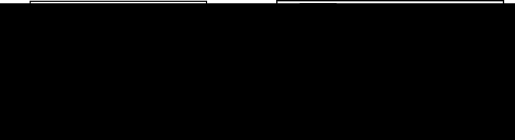
\includegraphics[width=.75\paperwidth]{../../dev/graphics/poster/gillespie.pdf}}
\end{frame}

\note[itemize]{
\item The kinetic monte carlo method, or the Gillespie Algorithm, was originally
developed to simulate stochastic chemical reactions. %TODO: This part feels like it would be better above
\item KMC is agnostic to what you're actually simulating, just cares about rates
\item %TODO: Do I even want to say the part about capturing the dynamics?
\item Time scale of a KMC step is not fixed and scales with number of reagents being
simulated. This is cool because as the system grows, and has more particles,
and therefore more frequent interactions, the time step gets shorter. This
simulates more reactions in the same amount of time. Conversely, the time step
will lengthen as the system shrinks.
\item Basic algorithm: Calculate likelihood of reaction happening, given size
of system, rates, and number of particles of each type. Use that probability
distribution to randomly select one. Choose a random timestep length from an
exponential distribution given by the number of particles.%TODO: Put the equations for this from the Rieger slides on a backup slide!
Carry out the reaction, updating the simulation with the result of the reaction.
}

%TODO: Well-Mixed "what"? Simulation? Case? Regime?
%TODO: Need to say more here about the two
\begin{frame}{Simulation Details}

  \begin{itemize}
    \item Slower plasmid carrier growth rate
    \item Carrying capacity
    \item Periodic boundary conditions
    \item Fixed death rate
    \item Mapping simulation time to real time%TODO: Write out what I want to say about mapping sim time to real time!
  \end{itemize}

\end{frame}
\begin{frame}{Simulation Detailed (cont'd)}

  Well-Mixed Case
  \begin{itemize}
    \item System-wide carrying capacity
    \item Most closely follows the model
  \end{itemize}

  Lattice Case
  \begin{itemize}
    \item Clustering
    \item Discrete sites with per-site carrying capacity
  \end{itemize}
\end{frame}
\note[itemize]{
\item%TODO: Add notes for this!
}

% \begin{frame}{Lattice}
% \end{frame}

\begin{frame}[fragile]{Optimizations}
  \begin{itemize}
    \item Occupancy lists
    \item Sets vs. lists
    \item \verb|imshow| vs. \verb|plcolor| %TODO: Does anyone care about this?
  \end{itemize}
\end{frame}
\note[itemize]{
\item When implemented for a lattice, the KMC algorithm goes pick a reaction THEN pick
a random site. So, we have to know which sites actually have the reagents necessary
for that reaction. Instead of searching through the whole lattice, which is very
slow, I just track a list of sites occupied by each type of particle. Then I can
just randomly pick from the appropriate list.

\item Sometimes it's hard to avoid searching through the array. For instance
when a transformation reaction happens, I need a site that's occupied by both
an S and a P. In order to get a list of those, I have to check which lattice sites
exist in both lists. However, that's a very slow operation. The way python
implements lists under the hood means that the time it takes to do that increases
with the square of the length of the lists, or the square of the lattice dimensions.
I use something called sets instead of lists, which are implemented in such a way
that the time it takes to do that same operation just goes linearly with the length
of the lists. (20x speedup with a small lattice)

\item plcolor and imshow are two ways of plotting, pcolor makes a whole array
of small squares where imshow just makes a picture. pcolor can look slightly
better but is orders of magnitude slower.
}




\section{Results}
\subsection{Well-Mixed}
\begin{frame}{Constant $\alpha$}
  \vspace*{3mm}
  \centerline{\includegraphics[width=.4\paperwidth]{../../dev/graphics/talk/const_contour.pdf}} %TODO: LABEL Z AXIS

  \begin{columns}
    \begin{column}{.5\paperwidth}
        \includegraphics[width=.5\paperwidth]{../../dev/graphics/talk/constant_population.pdf}
    \end{column}

    \vspace*{\fill}
    \begin{column}{.4\paperwidth}
      \textbf{Parameters} \\
      \begin{tabular}{l  r  c|c  l  r}
        \toprule
        $\alpha$ & .13 & \quad & \quad &
          $\frac{b_S}{b_R}$ & 1.07 \\
        $S_0$ & $10^3$ & \quad & \quad &
          $R_0$ & $10^3$ \\
        $P_0$ & $10^4$ & \quad & \quad &
          $K$ & $10^4$ \\
          \bottomrule
      \end{tabular}\\

      \redc{5pt}  Susceptible\\
      \bluec{5pt}  Resistant
    \end{column}
\end{columns}
\end{frame}

\begin{frame}{Linear $\alpha$}
  \vspace*{3mm}
  \centerline{\includegraphics[width=.4\paperwidth]{../../dev/graphics/talk/linear_contour.pdf}} %TODO: LABEL Z AXIS

  \begin{columns}
    \begin{column}{.5\paperwidth}
        \includegraphics[width=.5\paperwidth]{../../dev/graphics/talk/linear_population.pdf}
    \end{column}

    \vspace*{\fill}
    \begin{column}{.4\paperwidth}
      \textbf{Parameters} \\
      \begin{tabular}{l  r  c|c  l  r}
        \toprule
        $\alpha$ & .3 & \quad & \quad &
          $\frac{b_S}{b_R}$ & 1.07 \\
        $S_0$ & $10^3$ & \quad & \quad &
          $R_0$ & $10^3$ \\
        $P_0$ & $10^4$ & \quad & \quad &
          $K$ & $10^4$ \\
          \bottomrule
      \end{tabular}\\

      \redc{5pt}  Susceptible\\
      \bluec{5pt}  Resistant
    \end{column}
\end{columns}
\end{frame}

\begin{frame}{Recycled $\alpha$}
  \vspace*{3mm}
  \centerline{\includegraphics[width=.4\paperwidth]{../../dev/graphics/talk/recycled_contour.pdf}} %TODO: LABEL Z AXIS

  \begin{columns}
    \begin{column}{.5\paperwidth}
        \includegraphics[width=.5\paperwidth]{../../dev/graphics/talk/recycled_population.pdf}
    \end{column}

    \vspace*{\fill}
    \begin{column}{.4\paperwidth}
      \textbf{Parameters} \\
      \begin{tabular}{l  r  c|c  l  r}
        \toprule
        $\alpha$ & .13 & \quad & \quad &
          $\frac{b_S}{b_R}$ & 1.07 \\
        $S_0$ & $10^3$ & \quad & \quad &
          $R_0$ & $10^3$ \\
        $P_0$ & $10^4$ & \quad & \quad &
          $K$ & $10^4$ \\
          \bottomrule
      \end{tabular}\\

      \redc{5pt}  Susceptible\\
      \bluec{5pt}  Resistant
      \vfill
    \end{column}
\end{columns}
\end{frame}

\subsection{Lattice}
%TODO: What results do I want to show for the lattice?
% Show lattice plots vs model, and show huge differences.


\section{Conclusions}
\begin{frame}{Conclusions}
  \begin{alertblock}{What most heavily affects R or S dominance?}
    \begin{itemize}
      \item Transition point heavily dependent on $\alpha$
      \item Little growth rate dependence, except linear case
      % \item
    \end{itemize}
  \end{alertblock}

\end{frame}

%TODO: What other future work?
\begin{frame}{Future Work}
  \begin{itemize}
    \item Larger lattice simulations
    \item Simulate antibiotic dosing
    \item Incorporate diffusion reaction
  \end{itemize}

\end{frame}

%TODO: More? Move JJ from title to here? Which is appropriate
\begin{frame}{Acknowledgements}
Department of Physics and Astronomy, Bucknell University

NSF-DMR \#1248387

\vfill
\end{frame}

\begin{frame}[standout]
  Questions?
\end{frame}


\appendix

\begin{frame}{Gillespie Algorithm \footfullcite{rieger}}
  \begin{enumerate}
    \item Initialize simulation
    \item Calculate propensity $a$ for each reaction
    \item Choose reaction $\mu$ according to the distribution
      $$\text{P(reaction }\mu) = a_\mu / \sum_{i}a_i$$ %TODO: is this formatting ok?
    \item Choose time step length $\tau$ according to the distribution
      $$\text{P}(\tau)=\left(\sum_i a_i\right) \cdot \exp{\left(-\tau \sum_i ai\right)}$$
    \item Update populations with results of reaction
    \item Go to Step 2
  \end{enumerate}
\end{frame}

\begin{frame}[allowframebreaks]{References}
\end{frame}

\end{document}
